\documentclass[12pt]{book}
\usepackage[margin=.85in]{geometry} % for MARGIN
\usepackage[many]{tcolorbox}    	% for COLORED BOXES (tikz and xcolor included)


\usepackage{multicol}   
\usepackage{enumerate}
\usepackage[shortlabels]{enumitem}
\usepackage{varwidth}
\usepackage{tasks}
\usepackage[export]{adjustbox}

\usepackage{titleps}
\usepackage{setspace}               % for LINE SPACING
\usepackage[⟨options⟩]{fancyhdr}
\usepackage{enumitem}
\setlist{nosep}
\usepackage{tikz}
\usepackage{pgfplots}
\pgfplotsset{compat=1.5.1}
\usetikzlibrary{datavisualization}
\usetikzlibrary{datavisualization.formats.functions}

\newcommand{\D}{\displaystyle}


\setlength\parindent{0pt}   % killing indentation for all the text
\setstretch{1.3}            % setting line spacing to 1.3
\setlength\columnsep{0.25in} % setting length of column separator
\pagestyle{fancy}           % setting pagestyle to be headings

\usepackage[]{titlesec}

\fancyhead[L]{Math V04 - College Algebra}
\fancyhead[R]{Christina Papazacharioudakis}

\tcbset{
    sharp corners,
    colback = white,
    before skip = 0.2cm,    % add extra space before the box
    after skip = 0.5cm      % add extra space after the box
}                           % setting global options for tcolorbox

    \newtcolorbox{boxR}{
    fontupper = \color{black}, % font color
    boxrule = 1.5pt,
    colframe = black,
    rounded corners,
    arc = 5pt   % corners roundness
}

\definecolor{ballblue}{rgb}{0.13, 0.67, 0.8}

\begin{document}



\begin{comment}
Name: \underline{\hspace{100mm}}
\vspace{20mm}
  \centerline{\Large \textbf{Chapter 2: Equations and Inequalities} } 

{\large
\begin{center}
\begin{varwidth}{\textwidth}
\begin{enumerate}[2.1]
    \item The Regular Coordinate System and Graphs
    \item Linear Equations in One Variable
    \item Models and  Applications (Skipping)
    \item Complex Numbers
    \item Quadratic Equations
    \item Other Types of Equations
    \item Linear Inequalities and Absolute Value Inequalities
\end{enumerate}
\end{varwidth}
\end{center}

}
\newpage  
\end{comment}

{\Large \textbf{6.1 \& 6.2 Exponential Functions and Their Graphs}}
\vspace{3mm}

Chapter 6 looks at studying two new types of functions: exponential and logarithmic. We start with exponential functions which model lots of real world scenarios like tracking the population of a bacteria or the growth of a bank account gaining interest. So, what is an exponential function?
\vspace{3mm}

\begin{boxR}
    Exponential Function
    \vspace{1mm}
    \hline
    \vspace{2mm}
    The \textbf{exponential function $\mathbf{f(x)}$ with base $\mathbf{b}$} is defined by

    $$f(x)=ab^x \text{ or } y=ab^x$$
    where $a\neq0$, $b$ is a positive constant other than $1$ ($b >0$ and $b \neq 1$), and $x$ is any real number. 
\end{boxR}

Examples of exponential functions: 

\begin{multicols}{4}
    $f(x)=2^x$  \\ $g(x)=10^x$ \\ $h(x)=3^{x+1}$ \\ $j(x)=\left(\frac{1}{2}\right)^{x-1}$
\end{multicols}

\vspace{50mm}



  
\underline{\textbf{Example 1 - Evaluating Exponential Functions}}

The exponential function $f(x)=42.2(1.56)^x$ models the amount of money spent (in dollars) at a shopping mall after $x$ hours. How much money is spent on average after $4$ hours?


\newpage

\textbf{{\large Graphing Exponential Functions}}

When we are first learning what graphs of a function look like, a very first step we can take is plot points with a table. Let's go through this with an example.
\vspace{2mm}

\underline{\textbf{Example 2 - Graphing Exponential Functions}}

Make a table and plot the points for $f(x)=2^x$.

\begin{multicols}{2}
    

 \renewcommand{\arraystretch}{1.9} % Adjust row height for better vertical alignment
    \begin{tabular}{c|c} 
         $x$ & $f(x)=2^x$ \\
         \hline
         $-3$ &  \\ 
         \hline
         $-2$ &\\
         \hline
         $-1$ & \\
         \hline
         $0$ &  \\
         \hline
         $1$ &  \\
         \hline
         $2$ &  \\
         \hline
         $3$ &  \\
        \end{tabular}


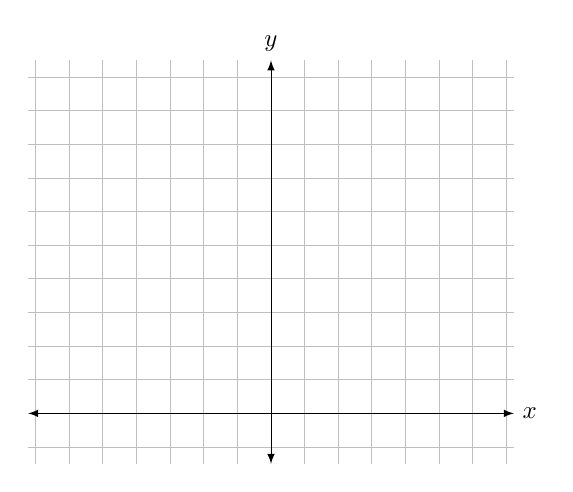
\begin{tikzpicture}[scale=0.9, transform shape]
\begin{axis}[
    ymin=-1.5,
    ymax=10.5,
    xmin=-3.5,
    xmax=3.5,
    axis on top=true,
    axis x line=middle,
    axis y line=middle,
    axis line style={latex-latex},
    xlabel=$x$,
    ylabel=$y$,
    xticklabels=\empty,
    yticklabels=\empty,
    xtick distance=1,
    ytick distance=1,
   xmajorgrids=true,
   ymajorgrids=true,
  axis equal = true, 
    every axis x label/.style={at={(ticklabel* cs:1.0)}, anchor=west,},
    every axis y label/.style={at={(ticklabel* cs:1.0)}, anchor=south,}
]
    \pgfplotsset{ticks=none}
\end{axis}
\end{tikzpicture}
\end{multicols}


\newpage
\underline{\textbf{Example 3 - Graphing Exponential Functions}}

Make a table and plot the points for $g(x)=\left(\frac{1}{2}\right)^x$.

Before we start the computations, let us note that: 

\vspace{15mm}
\begin{multicols}{2}
    

 \renewcommand{\arraystretch}{1.9} % Adjust row height for better vertical alignment
    \begin{tabular}{c|c} 
         $x$ & $f(x)=2^x$ \\
         \hline
         $-3$ &  \\ 
         \hline
         $-2$ &\\
         \hline
         $-1$ & \\
         \hline
         $0$ &  \\
         \hline
         $1$ &  \\
         \hline
         $2$ &  \\
         \hline
         $3$ &  \\
        \end{tabular}


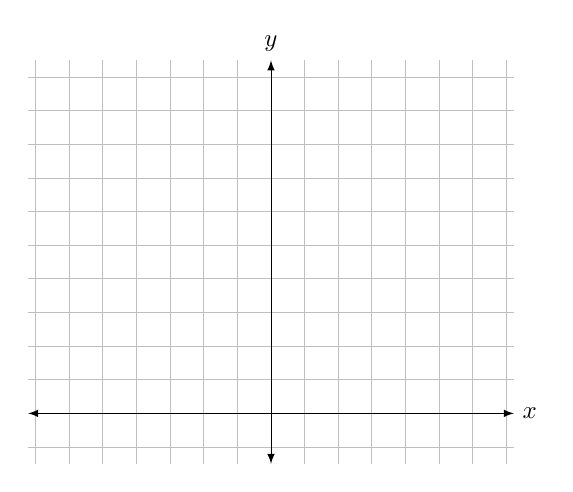
\begin{tikzpicture}[scale=0.9, transform shape]
\begin{axis}[
    ymin=-1.5,
    ymax=10.5,
    xmin=-3.5,
    xmax=3.5,
    axis on top=true,
    axis x line=middle,
    axis y line=middle,
    axis line style={latex-latex},
    xlabel=$x$,
    ylabel=$y$,
    xticklabels=\empty,
    yticklabels=\empty,
    xtick distance=1,
    ytick distance=1,
   xmajorgrids=true,
   ymajorgrids=true,
  axis equal = true, 
    every axis x label/.style={at={(ticklabel* cs:1.0)}, anchor=west,},
    every axis y label/.style={at={(ticklabel* cs:1.0)}, anchor=south,}
]
    \pgfplotsset{ticks=none}
\end{axis}
\end{tikzpicture}
\end{multicols}


\vspace{2mm}





\centerline{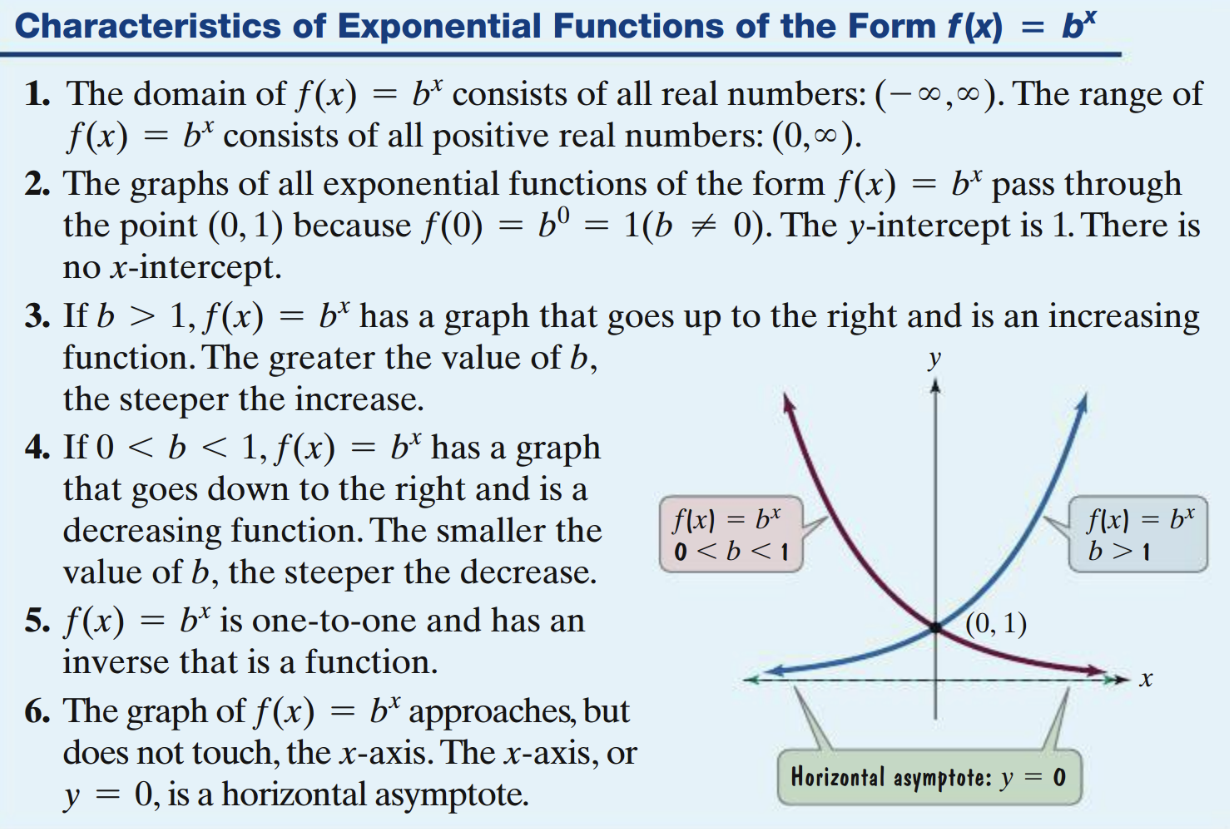
\includegraphics[scale=.6]{Chapter 6/6.1-figure1.png}}


\newpage


{\large \textbf{Transformations of Exponential Functions}}

Let's look at the graph of $f(x)=2^x$ and $g(x)=(\frac{1}{2})^x$ together.


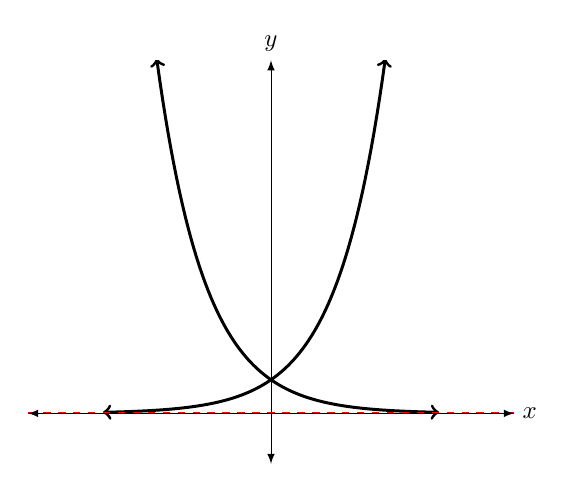
\begin{tikzpicture}[scale=0.9, transform shape]
\begin{axis}[
    ymin=-1.5,
    ymax=10.5,
    xmin=-5.5,
    xmax=5.5,
    axis on top=true,
    axis x line=middle,
    axis y line=middle,
    axis line style={latex-latex},
    xlabel=$x$,
    ylabel=$y$,
    xticklabels=\empty,
    yticklabels=\empty,
    xtick distance=1,
    ytick distance=1,
 %  xmajorgrids=true,
%   ymajorgrids=true,
  axis equal = true, 
    every axis x label/.style={at={(ticklabel* cs:1.0)}, anchor=west,},
    every axis y label/.style={at={(ticklabel* cs:1.0)}, anchor=south,}
]
 \pgfplotsset{ticks=none}
    \addplot [<->][very thick, samples=100, domain=-5:3.4] {2^x};
    \addplot [<->][very thick, samples=100, domain=-3.4:5] {2^(-1*x)};
    \addplot[dashed, thick, domain=-9:9,red] ({x},0.01);
\end{axis}
\end{tikzpicture}

How can we relate these graphs in terms of transformations of graphs? 

\vspace{20mm}

How can we graph $g(x)=3^{x} -1$ without plotting points? How about $h(x)=3^{x-4} +2$?

\centerline{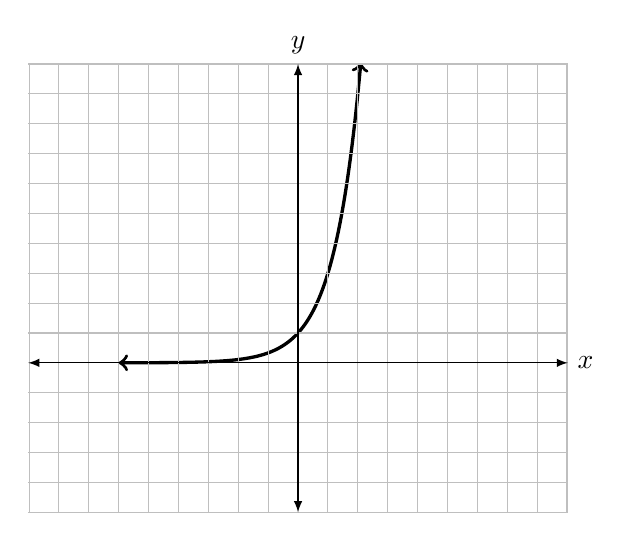
\begin{tikzpicture}[scale=1, transform shape]
\begin{axis}[
    ymin=-5,
    ymax=10,
    xmin=-5,
    xmax=5,
    axis on top=true,
    axis x line=middle,
    axis y line=middle,
    axis line style={latex-latex},
   % minor tick num=1,
   % major tick num=5,
    xlabel=$x$,
    ylabel=$y$,
   xticklabels=\empty,
  yticklabels=\empty,
   xtick distance=1,
    ytick distance=1,
  xmajorgrids=true,
 ymajorgrids=true,
     axis equal = true, 
    every axis x label/.style={at={(ticklabel* cs:1.0)}, anchor=west,},
    every axis y label/.style={at={(ticklabel* cs:1.0)}, anchor=south,}
]
    \pgfplotsset{ticks=none}
    \addplot [<->][very thick, samples=200, domain=-6:2.1] {3^x};
\end{axis}
\end{tikzpicture} }

\vspace{30mm}
Just as we applied transformations to the graph of our toolkit functions, we can apply transformations to exponential functions. 


\newpage

\centerline{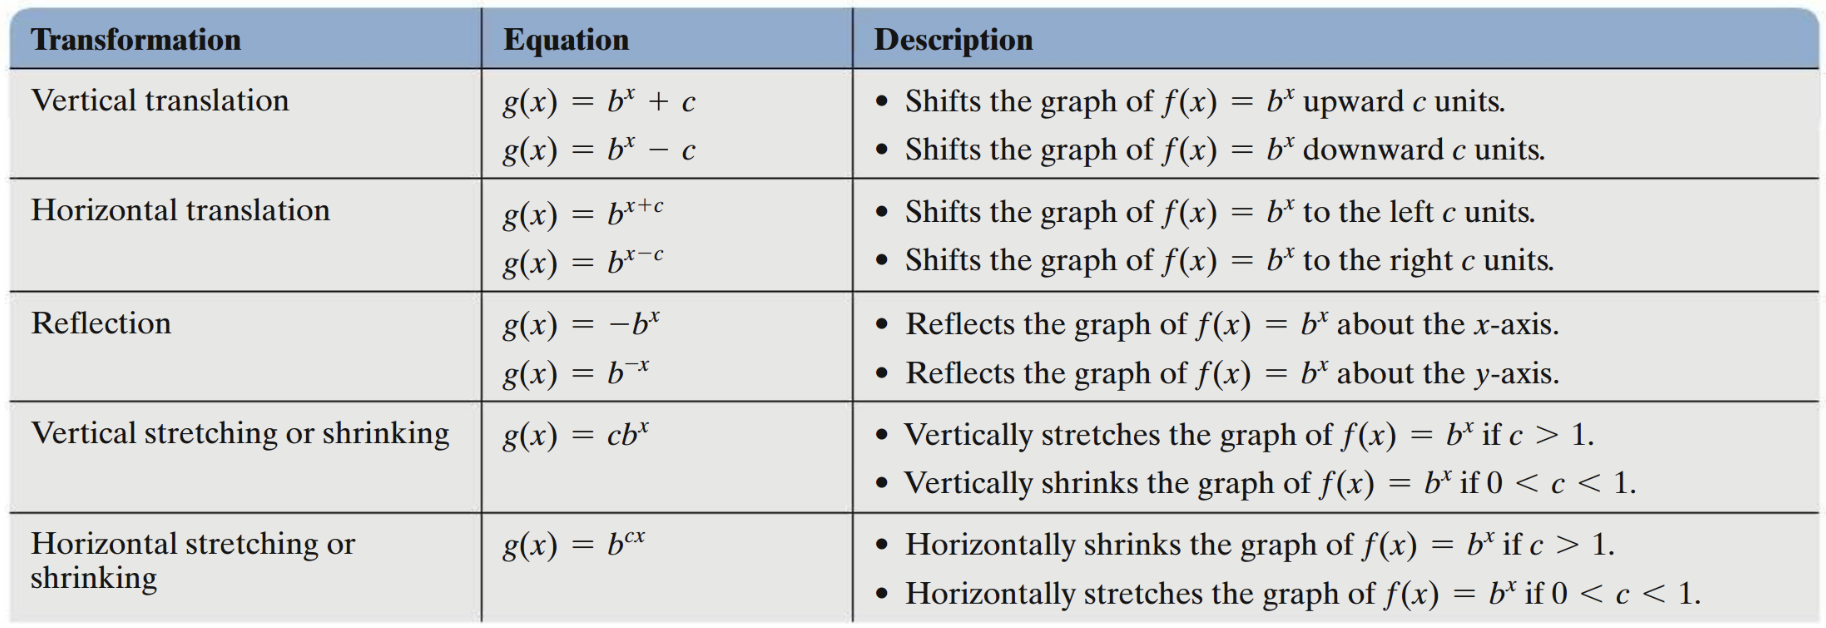
\includegraphics[scale=.6]{Chapter 6/6.1-figure2.png}}

\vspace{30mm}



{\large \textbf{The Natural Base $e$}}

An irrational number denoted by $e$ appears as the base in many applied exponential functions.

$$e \approx 2.718281827$$

We call $e\approx 2.72$ a \textbf{natural base} and $f(x)=e^x$ the \textbf{natural exponential function}.

\vspace{30mm}
\underline{\textbf{Example 4 - Using the Natural Exponential Function}}

The exponential function $f(x)=1144e^{0.0325x}$ models the population of gray wolves in the Western Great Lakes $x$ years after $1978$. According to the model, what is the population of gray wolves in $2018$?
\newpage

{\large \textbf{Using Exponential Functions for Compound Interest}}

Exponential functions can also help us track an account balance that is growing or accumulating interest.

\begin{boxR}
    \textbf{Formulas for Compound Interest}
    \vspace{1mm}
    \hline
    \vspace{2mm}

    After $t$ years, the balance, $A(t)$, in an account with an initial amount $P$ (principal amount) and an annual interest rate $r$ (in decimal form) is given by the following formulas:
\vspace{1mm}

    \begin{enumerate}
        \item For $n$ compounding periods per year: $\D A(t) = P\left(1+ \frac{r}{n}\right)^{nt}$
\vspace{1mm}
        \item For continuous compounding: $\D A(t)=Pe^{rt}$
    \end{enumerate}
\end{boxR}

\centerline{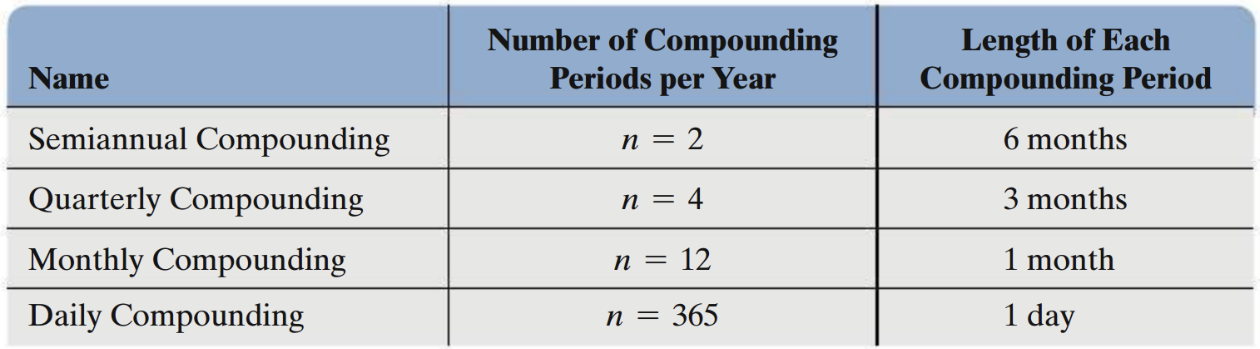
\includegraphics[scale=.7]{Chapter 6/6.1-figure3.png}}
\vspace{4mm}

\underline{\textbf{Example 5 - Calculating Compound Interest}}

If you invest $\$ 3,000$ in an investment account paying $3\%$ interest compounded quarterly, how much will the account be worth in $10$ years?


\newpage
\underline{\textbf{Example 6 - Choosing between Investments}}

You decided to invest $\$8000$ for $6$ years and you have a choice between two accounts. The first account pays $1.20\%$ per year, compounded monthly. The second pays $1.19\%$ per year, compounded continuously. Which is the better investment?




\newpage
    
        







\end{document}


